\section{Experiments on Image Source Separation}

\subsection{Image Decomposition}

In this section, we turn to use MMCA to separate two-dimensional data and compare the result with the standard FastICA source separation technique. \\

In Figure X, (a) and (d) are two source signals, one of which is oscillating textures while another is `boy' image. Curvelet transform is selected as the dictionary for source 1 and discrete consine transform is selected for source 2. Figure X (c) and (d) illustrates the separated image under the presence of 30dB gaussian noise.\\

The correlation coefficient between two sources are 0.07. It makes sense to ignore the correlation of source and ICA applies. We gradually apply noise from 0dB to 30dB. Correlation between source and separated image using MMCA and ICA methods is shown below.
The results proves the MMCA outperforms FastICA interms of separation quality and robustness.\\

(PSNR = 20dB) (using curvelet and DCT)
% -------------------------
\begin{figure*}
\centering
\subfigure[]{
\begin{minipage}[b]{0.23\linewidth}
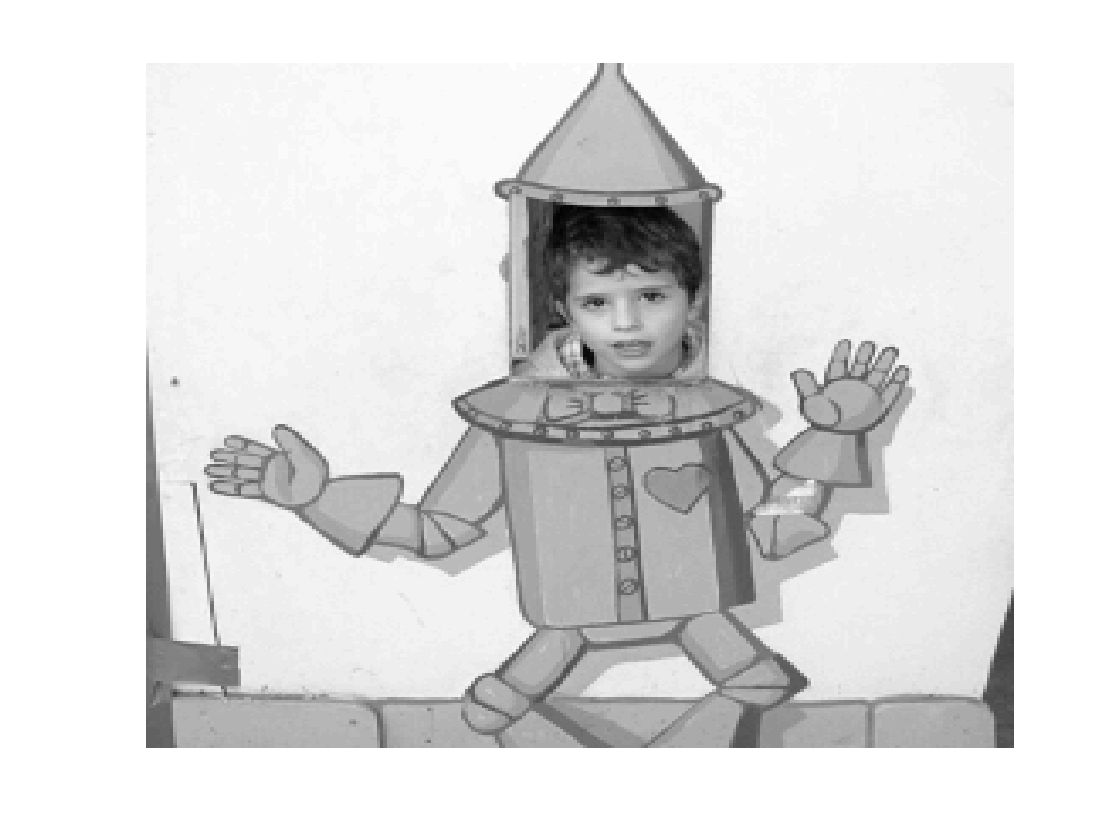
\includegraphics[width=1\linewidth]{images/source1.png}\vspace{4pt}
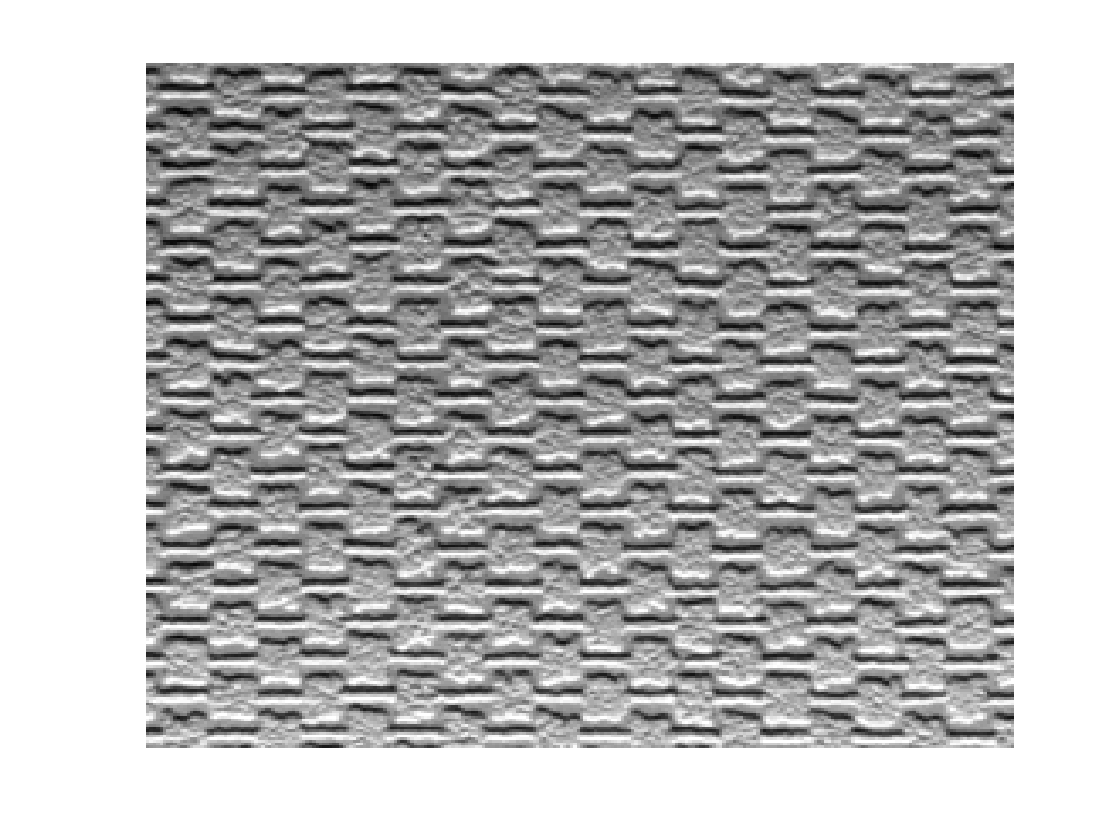
\includegraphics[width=1\linewidth]{images/source2.png}
\end{minipage}}
\subfigure[]{
\begin{minipage}[b]{0.23\linewidth}
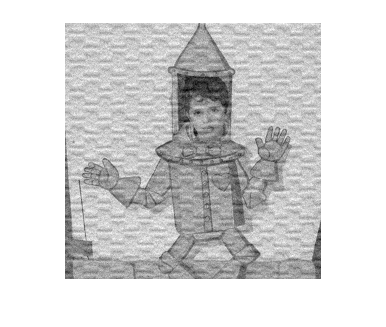
\includegraphics[width=1\linewidth]{images/separated1.png}\vspace{4pt}
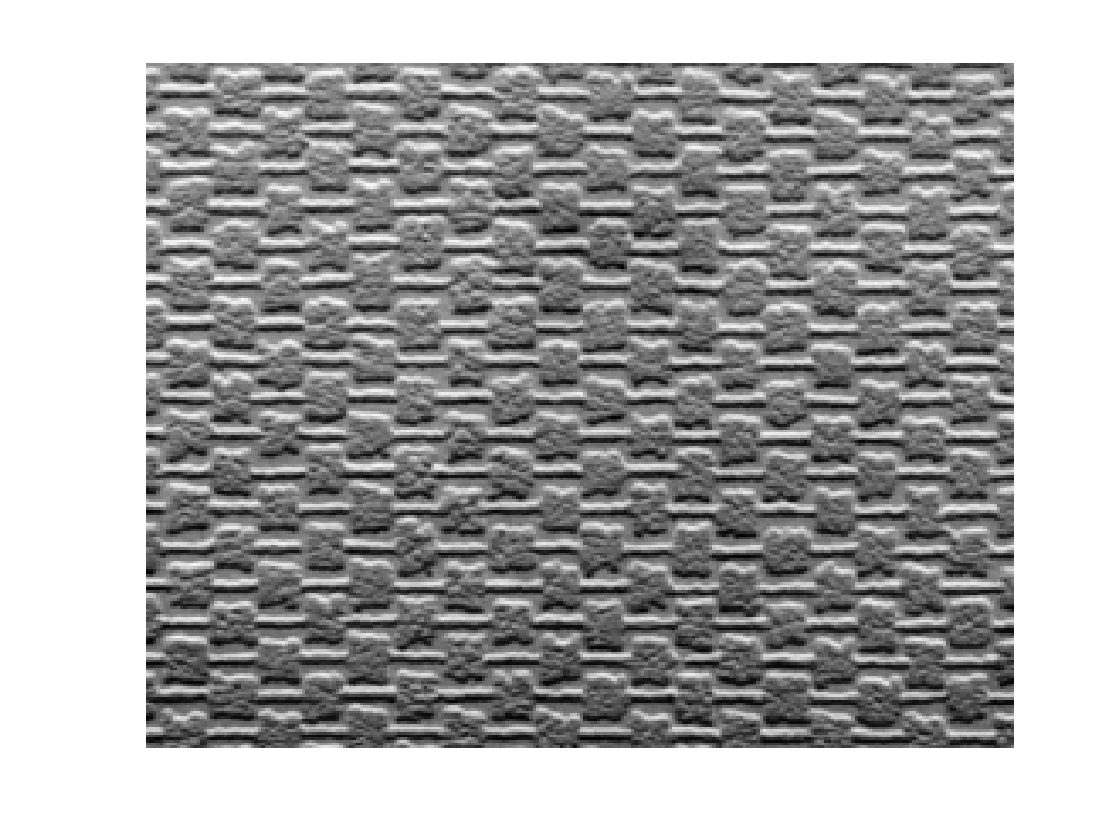
\includegraphics[width=1\linewidth]{images/separated2.png}
\end{minipage}}
\subfigure[]{
\begin{minipage}[b]{0.23\linewidth}
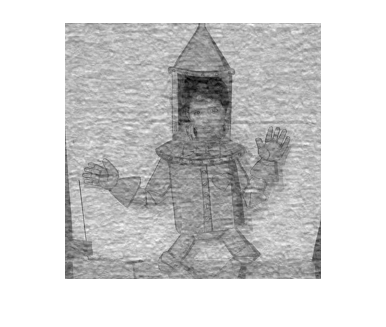
\includegraphics[width=1\linewidth]{images/MCA_Cartoon.png}\vspace{4pt}
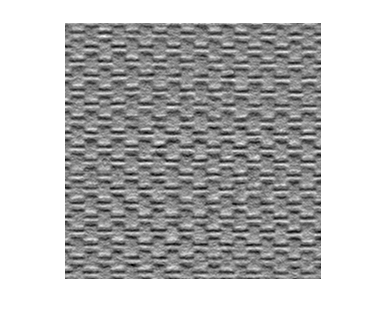
\includegraphics[width=1\linewidth]{images/MCA_Texture.png}
\end{minipage}}
\subfigure[]{
\begin{minipage}[b]{0.23\linewidth}
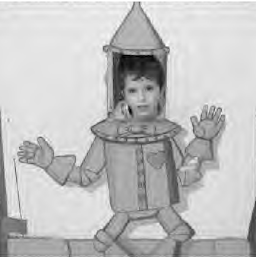
\includegraphics[width=1\linewidth]{images/mmca_cartoon.png}\vspace{4pt}
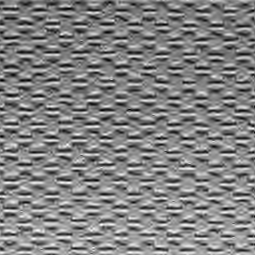
\includegraphics[width=1\linewidth]{images/mmca_texture.png}
\end{minipage}}

\caption{Experiment1: Image segmentation; \textbf{(a)}: Original sources; \textbf{(b)}: FastICA outputs; \textbf{(c)}: MCA outputs; \textbf{(d)}: MMCA outputs}
\end{figure*}
% -------------------------


\begin{figure}[!tbp]
\centering
\begin{minipage}[b]{0.85\textwidth}
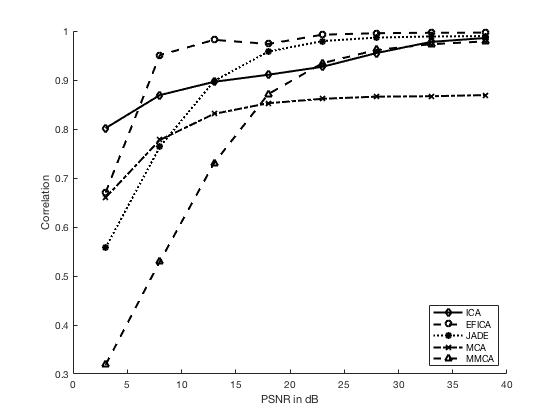
\includegraphics[width=\textwidth]{images/corr_plot_seg.png}
\caption{Evolution of the correlation coefficient between original and estimated sources as the noise variance varies.}
\end{minipage}

\begin{minipage}[b]{0.85\textwidth}
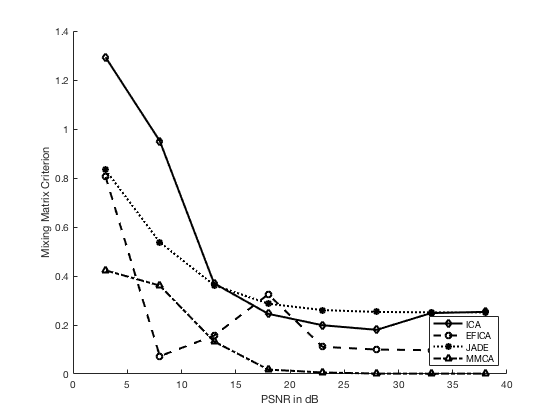
\includegraphics[width=\textwidth]{images/mmc_plot_seg.png}
\caption{Evolution of the mixing matrix criterion (after indeterminacy corrected) as the noise variance varies.}
\end{minipage}
\label{imapint1}
\end{figure}

\subsection{Blind Image Source Separation}

GMCA is supposed to achieve better separation quality when the mixing sources have similar morphologies. In this experiment, we use two scenery photo and compare GMCA with FastICA. Figure X (c) and (d) are two mixed signals. The result shows that both the two methods achieves good separation quality, but GMCA is slightly better. \\
In the robustness test, we impose guassian noise from 0dB to 30 dB. Figure X (c) and (d) are two mixed signals contaminated by 30dB noise. We can merely identify the original source from (e) and (f), but (c) and (d) using GMCA still gives acceptable result. It can also be shown in Figure X that noise has a greater effect on FastICA than GMCA. 


% ------------
\begin{figure*}
\centering
\subfigure[]{
\begin{minipage}[b]{0.23\linewidth}
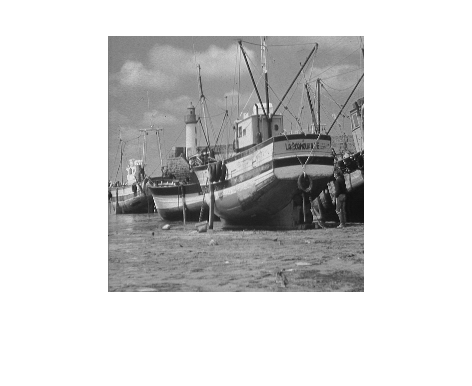
\includegraphics[width=1\linewidth]{images/boat_ori.png}\vspace{4pt}
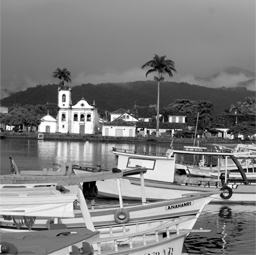
\includegraphics[width=1\linewidth]{images/paraty_ori.png}\vspace{4pt}
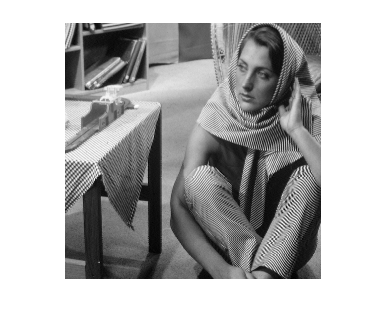
\includegraphics[width=1\linewidth]{images/barbara_ori.png}\vspace{4pt}
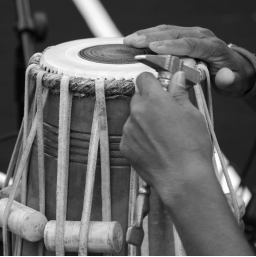
\includegraphics[width=1\linewidth]{images/pakhawaj_ori.png}
\end{minipage}}
\subfigure[]{
\begin{minipage}[b]{0.23\linewidth}
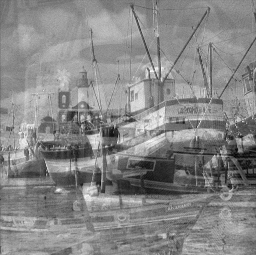
\includegraphics[width=1\linewidth]{images/efica_out1.png}\vspace{4pt}
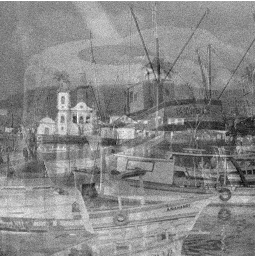
\includegraphics[width=1\linewidth]{images/efica_out2.png}\vspace{4pt}
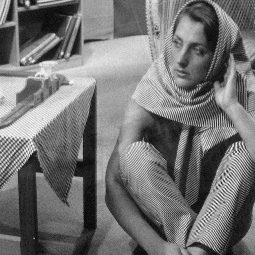
\includegraphics[width=1\linewidth]{images/efica_out3.png}\vspace{4pt}
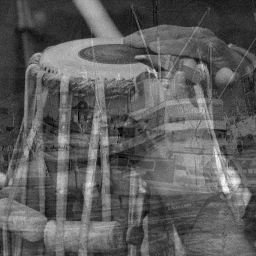
\includegraphics[width=1\linewidth]{images/efica_out4.png}
\end{minipage}}
\subfigure[]{
\begin{minipage}[b]{0.23\linewidth}
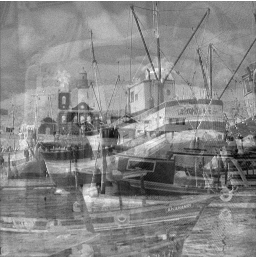
\includegraphics[width=1\linewidth]{images/jade_out1.png}\vspace{4pt}
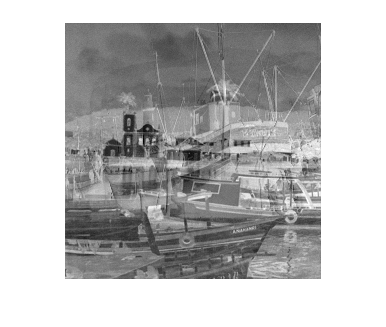
\includegraphics[width=1\linewidth]{images/jade_out2.png}\vspace{4pt}
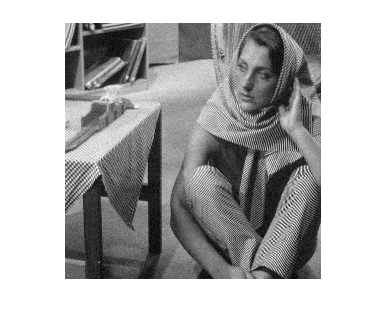
\includegraphics[width=1\linewidth]{images/jade_out3.png}\vspace{4pt}
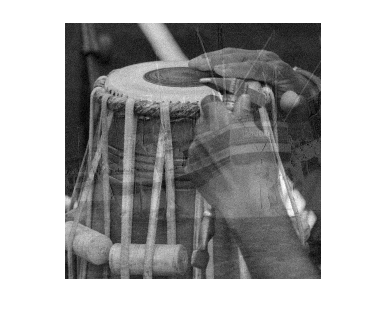
\includegraphics[width=1\linewidth]{images/jade_out4.png}
\end{minipage}}
\subfigure[]{
\begin{minipage}[b]{0.23\linewidth}
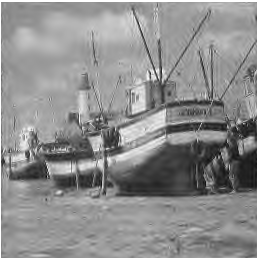
\includegraphics[width=1\linewidth]{images/gmca_out1.png}\vspace{4pt}
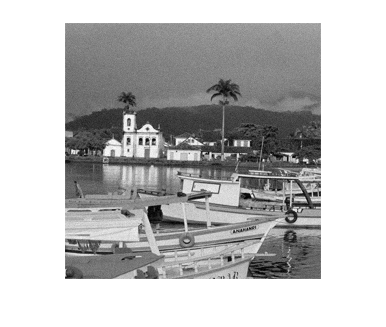
\includegraphics[width=1\linewidth]{images/gmca_out2.png}\vspace{4pt}
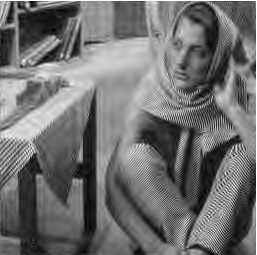
\includegraphics[width=1\linewidth]{images/gmca_out3.png}\vspace{4pt}
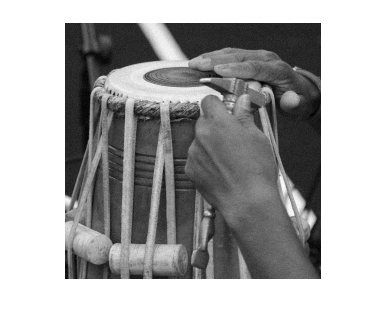
\includegraphics[width=1\linewidth]{images/gmca_out4.png}
\end{minipage}}
\caption{Experiment2: image separation; \textbf{(a)}:Original image sources; \textbf{(b)}:EFICA outputs; \textbf{(c)}:JADE outputs; \textbf{(d)}:GMCA outputs }
\end{figure*}
% ------------ 
 

\begin{figure}[!tbp]
\centering
\begin{minipage}[b]{0.85\textwidth}
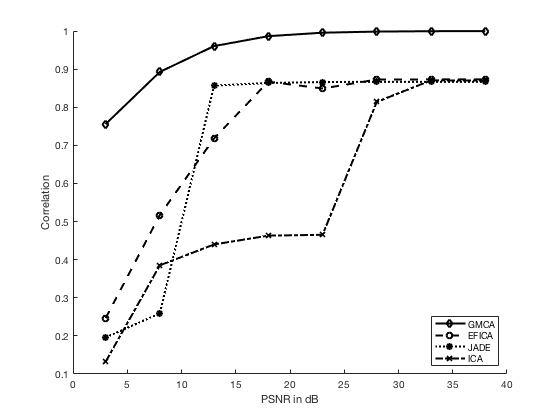
\includegraphics[width=\textwidth]{images/image_separation1.png}
\caption{Evolution of the correlation coefficient between original and estimated sources as the noise variance varies.}
\end{minipage}

\begin{minipage}[b]{0.85\textwidth}
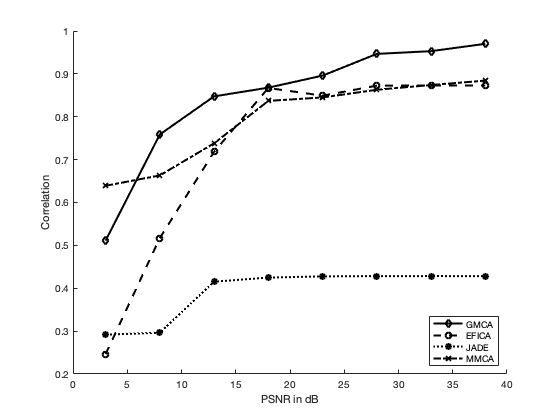
\includegraphics[width=\textwidth]{images/image_separation2.png}
\caption{Evolution of the mixing matrix criterion (after indeterminacy corrected) as the noise variance varies.}
\end{minipage}
\label{imapint1}
\end{figure}
